\documentclass[12pt,a4paper]{article}

\usepackage[T1]{fontenc}
\usepackage[spanish]{babel}
\usepackage{csquotes}
\usepackage{graphicx}
\usepackage{geometry}
\usepackage{pdflscape}
\usepackage{longtable}
\usepackage{array}
\setlength{\emergencystretch}{1em}
\usepackage[backend=biber,style=ieee,sorting=none,maxbibnames=99]{biblatex}
\DefineBibliographyStrings{spanish}{artno = {art\adddot}}
\AtBeginBibliography{\setlength{\emergencystretch}{1em}}
\addbibresource{referencias.bib}
\addbibresource{arquitectura/fuentes-arquitectura.bib}
\usepackage{xurl}
\usepackage[hidelinks]{hyperref}

% !TeX root = main.tex

% Escribe cada apartado dentro de su comando. Deja una línea en blanco
% entre párrafos. Para citar, usa \cite{clave} con la clave de referencias.bib.

% Punto 5 de la guía.
\newcommand{\CarlosTrabajosRelacionados}{%
  \section{Trabajos relacionados}

  Se comparan tres antecedentes para la aplicación de gestión de laboratorios
  informáticos (CLAB) de la Universidad Técnica Estatal de Quevedo (UTEQ).
  Gil Vera et al. presentan el \emph{STEM Real Remote Laboratory} (STEM RRL)
  \cite{gilVera2024}. García-Granja et al. desarrollan Biblio-Smart para la
  Biblioteca General de la Universidad de Málaga \cite{garciaGranja2022}.
  Müller et al. estudian el modelo del \emph{International Timetabling
  Competition 2019} (ITC 2019), construido a partir de datos de universidades que
  usan UniTime \cite{muller2025}. Las funciones de CLAB se presentan como
  propuestas de diseño. Su esqueleto actual demuestra la comunicación entre
  los servicios de Laboratorios y Reservas.

  \subsection{Recurso que se reserva}

  STEM RRL permite reservar acceso remoto a equipos físicos para prácticas de
  electrónica \cite{gilVera2024}. Biblio-Smart permite reservar un asiento
  individual de biblioteca \cite{garciaGranja2022}. El modelo de ITC 2019
  asigna aulas y franjas horarias a clases durante la planificación académica
  \cite{muller2025}. CLAB propone gestionar laboratorios informáticos completos
  para actividades presenciales. De STEM RRL puede tomar la identificación
  inequívoca del recurso reservado. De ITC 2019 puede aprovechar la relación
  entre espacio, franja y actividad para que cada reserva indique qué
  laboratorio se usará, cuándo y para qué.

  \subsection{Consulta de disponibilidad}

  En STEM RRL, el usuario elige un laboratorio remoto, un día y una franja
  habilitada en el calendario \cite{gilVera2024}. Biblio-Smart distingue en un
  mapa los asientos libres, reservados y ocupados, y permite consultar sus
  características antes de elegir \cite{garciaGranja2022}. ITC 2019 representa
  los periodos en los que cada aula puede asignarse \cite{muller2025}. CLAB
  propone un calendario por laboratorio que combine la selección por fecha de
  STEM RRL con la distinción visual de estados de Biblio-Smart. Un docente
  podría ver si una franja está disponible, reservada o bloqueada por la
  institución antes de enviar la solicitud.

  \subsection{Permisos según el usuario}

  STEM RRL asigna a estudiantes, docentes y administradores permisos diferentes
  para reservar, configurar equipos o programar mantenimiento
  \cite{gilVera2024}. Biblio-Smart ofrece un flujo de reserva para los miembros
  de la universidad a través de su aplicación institucional
  \cite{garciaGranja2022}. ITC 2019 emplea matrículas y grupos para determinar
  a qué clases puede asignarse cada estudiante dentro del horario
  \cite{muller2025}. CLAB puede tomar de STEM RRL la separación entre quienes
  solicitan una franja y quienes administran la disponibilidad. Esa distinción
  permite definir quién puede solicitar una reserva, programar una serie o
  bloquear un laboratorio, de acuerdo con las responsabilidades de la UTEQ.

  \subsection{Reservas puntuales y recurrentes}

  STEM RRL permite reservar franjas por adelantado y ofrece a los docentes
  la opción de programar reservas periódicas \cite{gilVera2024}.
  Biblio-Smart describe la reserva individual de un asiento con un plazo
  para ocuparlo \cite{garciaGranja2022}. ITC 2019 admite clases que se repiten
  varios días o únicamente en determinadas semanas del semestre
  \cite{muller2025}. CLAB propone cubrir tanto una práctica puntual como una
  asignación recurrente para una materia. De STEM RRL puede tomar la
  distinción entre ambos flujos y de ITC 2019 puede aprovechar el manejo de
  excepciones, como omitir una fecha en la que el laboratorio esté bloqueado.

  \subsection{Conflictos y alternativas de horario}

  STEM RRL marca las franjas reservadas por otros usuarios y exige que los
  bloques de una misma selección sean contiguos \cite{gilVera2024}.
  Biblio-Smart permite consultar los atributos de distintos asientos libres
  para elegir el que mejor se ajuste a las necesidades del usuario
  \cite{garciaGranja2022}. ITC 2019 distingue las restricciones obligatorias
  de las preferencias al evaluar un horario \cite{muller2025}. CLAB podría
  aplicar esa distinción a cada solicitud. Un solapamiento con una reserva
  confirmada del mismo laboratorio impediría aceptarla. La cercanía a la hora
  solicitada serviría para ordenar las alternativas disponibles. La regla
  contra solapamientos también tendría que verificarse con solicitudes
  simultáneas cuando se implemente la reserva.

  \subsection{Confirmación y uso efectivo del recurso}

  STEM RRL genera una credencial asociada a la reserva para acceder al equipo
  remoto durante la franja asignada \cite{gilVera2024}. Biblio-Smart envía una
  confirmación por correo, detecta la presencia del usuario en el asiento
  mediante el teléfono y libera el puesto después del periodo de ausencia
  configurado \cite{garciaGranja2022}. ITC 2019 genera una asignación que indica
  dónde y cuándo debe realizarse cada clase \cite{muller2025}. CLAB podría
  tomar de Biblio-Smart la distinción entre una reserva confirmada y el uso
  efectivo del espacio. Si el alcance incluye un registro de asistencia, esa
  distinción permitiría identificar qué reservas llegaron a utilizarse.

  \subsection{Bloqueos y cambios de disponibilidad}

  STEM RRL permite habilitar o deshabilitar recursos, fijar sus periodos de
  disponibilidad y programar mantenimiento \cite{gilVera2024}. Biblio-Smart
  actualiza el estado de los asientos según la reserva y la presencia del
  usuario. También simula cómo una regla de distanciamiento cambia los
  puestos disponibles \cite{garciaGranja2022}. ITC 2019 admite periodos en
  los que un aula no puede asignarse \cite{muller2025}. CLAB podría combinar
  el caso de mantenimiento de STEM RRL con los periodos no disponibles de
  ITC 2019 para bloquear un laboratorio durante una franja concreta. Cuando
  un bloqueo afecte una reserva confirmada, el flujo tendría que contemplar
  cómo avisar al responsable y gestionar la reprogramación.

  \subsection{Arquitectura e integración}

  STEM RRL conecta un sistema de reservas independiente con la plataforma
  académica y los equipos de acceso remoto \cite{gilVera2024}. Biblio-Smart
  combina una aplicación móvil, un servicio web, dispositivos de detección
  y un modelo digital del edificio \cite{garciaGranja2022}. ITC 2019 usa
  datos exportados de UniTime para comparar algoritmos que generan horarios
  \cite{muller2025}. En el esqueleto de CLAB, Reservas consulta a
  Laboratorios mediante REST con JSON. El proyecto puede tomar de STEM RRL
  la separación entre la gestión del recurso y la de sus reservas, y de
  Biblio-Smart la idea de presentar el estado del recurso de forma clara
  en la interfaz.

  \subsection{Evaluación del sistema}

  STEM RRL recogió comentarios de 28 estudiantes después de probar el
  laboratorio remoto en tres prácticas, con preguntas sobre la reserva y el
  acceso \cite{gilVera2024}. Biblio-Smart obtuvo 242 respuestas completas y
  voluntarias sobre la calidad percibida del prototipo y la información de
  los asientos \cite{garciaGranja2022}. ITC 2019 comparó algoritmos con 30
  casos de planificación universitaria, entre ellos uno de Yachay Tech,
  Ecuador, y examinó los resultados de asignación y los tiempos de cómputo
  \cite{muller2025}. CLAB podría adoptar dos formas de evaluación. Con usuarios
  de la UTEQ, comprobar si pueden encontrar y solicitar una franja. Con
  pruebas técnicas, verificar que las reglas se cumplan en reservas
  simultáneas, recurrentes y afectadas por bloqueos.
}

% Punto 6 de la guía, dentro de la sección de requisitos del equipo.
\newcommand{\CarlosRequisitosNoFuncionales}{%
  \subsection{Requisitos no funcionales}

  Estos requisitos describen cómo deberá comportarse la versión distribuida de
  CLAB cuando estén implementadas las funciones que se evalúan. Se clasifican
  según el modelo de calidad de
  \href{https://www.iso.org/standard/78176.html}{ISO/IEC 25010:2023}.
  Los 50 usuarios concurrentes, los 2 segundos y el 99\,\% de disponibilidad
  proceden del informe previo de CLAB. La configuración de las pruebas y los
  demás umbrales son propuestas que el equipo deberá validar con el
  levantamiento de información.

  \paragraph{RNF-01. Tiempo de respuesta (eficiencia de desempeño).}
  Durante 10 minutos de carga estable con 50 usuarios virtuales concurrentes,
  al menos el 95\,\% de las consultas válidas de disponibilidad deberá
  devolver el resultado correcto en menos de 2 segundos. La medición se
  realizará desde el cliente de prueba y el cálculo incluirá todas las
  consultas emitidas, contando las respuestas erróneas y los tiempos de
  espera agotados como incumplimientos. Para repetir la prueba se registrarán
  la configuración del entorno, los datos de la agenda y el perfil de carga.
  El uso de percentiles bajo distintos niveles de concurrencia se apoya en
  \cite{pantelic2026Carga}.

  \paragraph{RNF-02. Disponibilidad de la agenda (fiabilidad).}
  Durante dos semanas, dentro del horario académico acordado con la UTEQ, al
  menos el 99\,\% de las comprobaciones programadas de disponibilidad deberá
  devolver un resultado correcto antes de agotar un tiempo de espera de
  5 segundos. Una sonda externa al servicio ejecutará una consulta por minuto
  con una cuenta de prueba autorizada. La tasa se calculará dividiendo las
  comprobaciones exitosas por las programadas en la ventana de observación.
  Se toma como referencia el uso de comprobaciones externas para medir la
  disponibilidad \cite{mulahuwaish2022Disponibilidad}.

  \paragraph{RNF-03. Autorización de operaciones (seguridad).}
  En el 100\,\% de los casos de prueba de confirmación, cancelación y bloqueo,
  la operación deberá quedar sin ejecutar si el usuario carece del permiso,
  la sesión se ha revocado o el servicio de Identidad no puede verificar la
  autorización. Se probará cada operación en esas tres condiciones y se
  comprobará, además de la respuesta, que el estado de la agenda se conserve.
  Los estudios sobre control de acceso y revocación sustentan la verificación
  de estos escenarios
  \cite{venckauskas2023Autorizacion,rasori2024Revocacion}.

  \paragraph{RNF-04. Interfaz en escritorio y móvil (capacidad de interacción).}
  Una persona con permisos deberá poder completar la consulta de disponibilidad
  y el envío de una solicitud en las seis combinaciones de Chrome, Firefox y
  Edge con anchos de pantalla de 360 y 1280 píxeles. En cada combinación
  deberán poder utilizarse los controles necesarios de ambos flujos sin
  desplazamiento horizontal de la página. La prueba registrará la versión
  de cada navegador y el resultado de los dos flujos para cada ancho.
  La evaluación en distintas configuraciones se apoya en el estudio de
  incompatibilidades de presentación \cite{watanabe2023Interfaz}.

  \paragraph{RNF-05. Instalación institucional (flexibilidad).}
  El 100\,\% de los servicios incluidos en la versión evaluada deberá poder
  desplegarse en un entorno limpio, con los prerrequisitos documentados,
  equivalente al entorno institucional. Una vez instalados los servicios,
  la prueba deberá completar una consulta de disponibilidad y confirmar una
  reserva con el acceso a servicios de nube pública deshabilitado.
  El procedimiento toma como referencia la instalación local reproducible
  de una aplicación de microservicios \cite{simoes2026Despliegue}.

  \paragraph{RNF-06. Continuidad ante la caída de Avisos (fiabilidad).}
  Con Información y Avisos detenido y las dependencias de la agenda operativas,
  las 10 solicitudes válidas de la prueba, cada una para una franja libre
  diferente, deberán confirmarse y quedar guardadas en Reservas y Agenda.
  Se comprobará la confirmación y la persistencia de cada solicitud antes
  de restablecer el servicio detenido. Este escenario aplica la evaluación
  mediante fallos inducidos a una dependencia concreta de CLAB
  \cite{alSaidAhmad2024Fallos}.

  \paragraph{RNF-07. Trazabilidad de cambios de agenda (seguridad).}
  El 100\,\% de las confirmaciones, cancelaciones y bloqueos exitosos del
  conjunto de prueba deberá tener un registro de auditoría en el servicio
  de origen. El registro deberá contener el identificador de la operación,
  el usuario, la acción y la fecha y hora. Se cotejará cada cambio con su
  registro tanto con la vista central de auditoría activa como durante su
  caída. Los datos del registro se apoyan en el modelo de trazabilidad de
  eventos de \cite{lopezPimentel2022Auditoria}.
}

% Punto 12 de la guía.
\newcommand{\CarlosRiesgosTecnicos}{%
  \section{Análisis de riesgos}

  El \href{https://github.com/ereinosov/app-dist-form-ac-01/blob/fccfe3f42f0cfa3c405825c4c642b5a5cbfa052b/FORM-AC-01/main.pdf}{informe de FORM-AC-01}
  analiza la caída de Amazon S3 en la región US-EAST-1 del 28 de febrero de
  2017. El \href{https://aws.amazon.com/message/41926/}{informe oficial de AWS}
  documenta tres lecciones que se aplican a CLAB: limitar el alcance de las
  operaciones de mantenimiento, mantener disponible un canal para comunicar
  incidentes y ensayar la recuperación de los componentes críticos. Los
  primeros tres riesgos derivan de ese caso. Los dos restantes surgen de la
  arquitectura propuesta en ADR-001.

  La valoración es cualitativa y corresponde al escenario previo a aplicar
  las mitigaciones. La probabilidad se considera media cuando el escenario
  puede surgir en tareas habituales de mantenimiento, uso o recuperación,
  y baja cuando requiere un fallo excepcional. El impacto es alto si se
  interrumpe la agenda o se compromete la integridad de sus datos. Se considera
  medio si se afecta el diagnóstico o la información secundaria y la agenda
  conserva sus datos. Las verificaciones se proponen para un entorno de
  pruebas con datos de prueba.

  \paragraph{R-01. Bloqueo de la agenda por una operación de mantenimiento.}
  En S3, un parámetro incorrecto permitió retirar más capacidad de la
  prevista. La tabla~2 de FORM-AC-01 traslada esta lección a CLAB: una
  operación de mantenimiento que retenga bloqueos en PostgreSQL podría
  agotar las conexiones de Reservas y Agenda. \textbf{Probabilidad media}
  por la ejecución prevista de tareas de mantenimiento.
  \textbf{Impacto alto} porque se podrían interrumpir las consultas y
  confirmaciones. La mitigación consiste en separar las credenciales de
  la aplicación y de mantenimiento, limitar los permisos y el alcance de
  cada operación, y acotar las esperas por bloqueos y conexiones. Para
  verificarla se mantendrá un bloqueo controlado en la base de pruebas.
  Se comprobará que la API devuelva un error dentro del límite configurado,
  que la solicitud afectada no quede confirmada y que las consultas se
  recuperen al liberar el bloqueo.

  \paragraph{R-02. Pérdida del canal de estado durante una caída.}
  La consola que permitía actualizar el panel de estado de AWS dependía
  del propio S3. En CLAB, si la detección y la comunicación de incidentes
  dependieran de la misma base que usa la agenda, el equipo podría perder
  ambas al mismo tiempo. \textbf{Probabilidad media} por la posibilidad de
  compartir infraestructura. \textbf{Impacto medio} porque retrasaría el
  diagnóstico y el aviso a los usuarios. La mitigación es ejecutar la sonda
  de RNF-02 desde fuera de la aplicación y acordar un canal institucional
  de aviso que pueda usarse durante la caída. Se verificará deteniendo
  PostgreSQL en el entorno de pruebas y comprobando que la sonda registre
  la indisponibilidad y que el aviso pueda emitirse por el canal alterno.

  \paragraph{R-03. Recuperación lenta o incompleta de la agenda.}
  En S3, el reinicio completo y la validación de metadatos tardaron más
  de lo previsto. En CLAB, una recuperación completa de PostgreSQL podría
  tardar más de lo esperado o devolver una agenda que requiera comprobaciones
  adicionales. \textbf{Probabilidad baja} porque el escenario requiere
  una interrupción que obligue a recuperar el almacén completo.
  \textbf{Impacto alto} por la posible interrupción prolongada de las
  confirmaciones. La mitigación es ensayar el procedimiento de recuperación
  y verificar la agenda antes de habilitar de nuevo las escrituras. Se
  restaurará una copia conocida, se medirá el tiempo hasta recuperar una
  consulta y una confirmación correctas, y se cotejarán las reservas y
  bloqueos recuperados con los datos esperados de esa copia.

  \paragraph{R-04. Confirmación de reservas superpuestas.}
  Si dos solicitudes concurrentes validan la misma franja antes de que
  se guarde la primera, ambas podrían confirmarse. \textbf{Probabilidad
  media} porque varios usuarios pueden solicitar el mismo laboratorio.
  \textbf{Impacto alto} porque se asignaría un espacio a actividades
  incompatibles. Según ADR-001, Reservas y Agenda debe serializar las
  modificaciones por laboratorio y verificar los solapamientos dentro de
  la misma transacción que guarda el cambio. Se enviarán dos solicitudes
  válidas para el mismo laboratorio y franja, y se comprobará que quede
  una sola reserva confirmada. Se repetirá la prueba con una reserva frente
  a un bloqueo para comprobar que no queden ambos vigentes.

  \paragraph{R-05. Avisos omitidos o duplicados al recuperar el servicio.}
  Si Información y Avisos se detiene mientras consulta los cambios de la
  agenda, podría omitir un evento pendiente o procesarlo dos veces al
  reiniciar. \textbf{Probabilidad media} porque una interrupción puede
  coincidir con el procesamiento. \textbf{Impacto medio} porque los
  usuarios podrían recibir avisos repetidos o consultar una vista de
  auditoría incompleta. La mitigación propuesta en ADR-001 consiste en
  conservar un registro durable en el servicio de origen, guardar el
  avance del consumidor y deduplicar por origen e identificador. Se
  detendrá Información y Avisos, se confirmarán reservas durante el corte
  y, al reanudarlo, se comprobará que cada evento pendiente se refleje
  una sola vez. La prueba complementa RNF-06 y RNF-07.
}

% !TeX root = main.tex

\newcommand{\ByronPortada}{%
  \begin{titlepage}
    \fontsize{12}{14}\selectfont
    \renewcommand{\arraystretch}{1.3}
    \centering
    {\Large\bfseries Universidad Técnica Estatal de Quevedo\par}
    \vspace{0.4cm}
    Facultad de Ciencias de la Computación\par
    Carrera de Software\par
    \vspace{1.2cm}
    {\Large\bfseries CLAB\par}
    \vspace{0.3cm}
    {\large Sistema distribuido de gestión de laboratorios\par}
    \vspace{0.8cm}
    \textbf{Proyecto Fin de Curso, entrega 1}\par
    Definición, requisitos y arquitectura base del sistema distribuido\par
    \vspace{0.8cm}
    TA-PFC-E1\par
    Aplicaciones Distribuidas (ISR-701)\par
    Séptimo nivel, paralelo A\par
    Periodo académico regular 2026-2027 SPA\par
    \vspace{0.8cm}
    \begin{tabular}{|p{0.43\textwidth}|p{0.43\textwidth}|}
      \hline
      \textbf{Integrante} & \textbf{Rol} \\ \hline
      Byron Daniel Loor Mendoza & Responsable de Documentación \\ \hline
      Roger Garcia & Arquitecto \\ \hline
      Juliana Emanuel Pino & Líder de Desarrollo \\ \hline
      Carlos Manotoa & Responsable de Calidad \\ \hline
    \end{tabular}
    \vspace{0.8cm}

    \textbf{Docente}\par
    Gleiston Cicerón Guerrero Ulloa\par
    \vspace{0.6cm}
    \textbf{Entrega prevista}\par
    29 de noviembre de 2026\par
    \vspace{0.6cm}
    \textbf{Repositorio del proyecto}\par
    \url{https://github.com/Danxxx777/clab-pfc-7a}\par
    \vfill
    Quevedo, Los Ríos, Ecuador\par
  \end{titlepage}
}

\newcommand{\ByronResumen}{%
  \section*{Resumen ejecutivo}
  CLAB es un proyecto universitario orientado a la gestión de los laboratorios
  informáticos de la Facultad de Ciencias de la Computación de la Universidad
  Técnica Estatal de Quevedo. El informe original describe reservas coordinadas
  por correo o mensajería, inventarios en hojas de cálculo, reportes verbales de
  fallas y dificultades para disponer de información consolidada sobre el uso
  de los espacios. Ese antecedente documenta una aplicación con Angular,
  Spring Boot y PostgreSQL y sirve como punto de partida para su evolución
  durante el Proyecto Fin de Curso de Aplicaciones Distribuidas
  \cite[pp.~4--5, 19--20]{clabAntecedente2026}.

  Los usuarios previstos son docentes, coordinadores de carrera, administradores
  de laboratorio y administradores del sistema. Los docentes consultarán la
  disponibilidad, gestionarán reservas y comunicarán fallas. La coordinación
  académica utilizará la agenda y los reportes para planificar el uso de los
  laboratorios. La administración de laboratorio mantendrá el catálogo y el
  inventario, mientras que la administración del sistema gestionará accesos,
  permisos y bloqueos institucionales.

  La arquitectura propuesta agrupa los módulos del legado en cuatro servicios
  por dominio, Identidad y Académico, Laboratorios y Recursos, Reservas y Agenda,
  e Información y Avisos. La distribución busca permitir despliegues
  independientes y aislar el procesamiento de reportes y notificaciones de la
  confirmación de reservas. Cada servicio tendrá almacenamiento de su propiedad.
  La agenda conservará una autoridad sobre la ocupación para evitar
  confirmaciones incompatibles. Estas decisiones se contrastarán con los
  requisitos de calidad y con el costo de introducir dependencias de red.

  El alcance académico se organiza en cuatro entregas. E1 establece los
  requisitos y la arquitectura y demuestra la comunicación entre dos procesos.
  E2 desarrollará las API y la contenerización. E3 abordará los datos y el
  procesamiento distribuido. E4 completará la integración, las pruebas y la
  observabilidad. El esqueleto actual permite consultar Laboratorios desde
  Reservas y observar un error cuando la dependencia está detenida.

  La validación combinará criterios funcionales, pruebas de concurrencia y
  mediciones de calidad. El diagnóstico del informe previo se conserva como
  antecedente. Su vinculación con el acta firmada o la grabación consentida
  exigida por E1 y la aprobación del alcance por el equipo siguen pendientes.
}

\newcommand{\ByronContexto}{%
  \section{Contexto y problema}
  \subsection{Organización y antecedente}
  El dominio del proyecto son los laboratorios informáticos de la Facultad de
  Ciencias de la Computación de la UTEQ. El informe original de CLAB identifica
  cuatro necesidades relacionadas, la coordinación de reservas, el inventario
  de equipos, el seguimiento de incidencias y la consulta de información para
  la planificación institucional \cite[pp.~4--5, 19--20]{clabAntecedente2026}.
  La versión desarrollada en semestres anteriores se consulta en el
  \href{https://github.com/Danxxx777/Clab--Sistema}{repositorio original de CLAB}.
  E1 parte de ese antecedente para definir la evolución
  distribuida y delimitar sus servicios.

  \subsection{Diagnóstico documentado}
  El informe previo describe reservas por correo electrónico y mensajería,
  con conflictos detectados al llegar al laboratorio. También reporta
  inventarios en archivos Excel sin una versión centralizada, fallas
  comunicadas verbalmente y falta de información estructurada para las
  decisiones de mantenimiento e inversión
  \cite[pp.~19--20]{clabAntecedente2026}.

  Como consecuencias, el documento señala pérdida de tiempo de clase,
  planificación con equipos fuera de servicio, reportes duplicados y
  mantenimiento reactivo. El intervalo de consulta de disponibilidad se
  describe cualitativamente como horas o días. Esa afirmación no aporta una
  muestra de tiempos ni un registro de mediciones. Para cuantificar el impacto
  se requiere conservar la fecha de cada solicitud y confirmación, la cantidad
  de conflictos y los tiempos de atención de incidencias. Esas mediciones
  siguen pendientes para la evaluación de E1.

  \subsection{Interesados identificados en el antecedente}
  Los perfiles y sus expectativas se obtienen de los requisitos y casos de uso
  del informe original \cite[pp.~14--15, 20, 25--32]{clabAntecedente2026}.
  \begin{description}
    \item[Docentes.] Consultar la agenda, gestionar sus reservas y registrar
    fallas de los equipos utilizados en las clases.
    \item[Coordinación de carrera.] Planificar el uso académico de los
    laboratorios, resolver conflictos y consultar reportes por carrera y periodo.
    \item[Administración de laboratorio.] Mantener el inventario y el estado
    de los recursos, atender incidencias y registrar asistencia.
    \item[Administración del sistema.] Gestionar usuarios y permisos,
    registrar bloqueos institucionales y consultar la auditoría.
  \end{description}

  \subsection{Respaldo del levantamiento}
  El Anexo A del informe contiene el cuestionario para autoridades, docentes y
  administradores. El Anexo B incluye una fotografía identificada como
  evidencia de entrevistas \cite[pp.~45--47]{clabAntecedente2026}. La copia
  recibida se conserva sin modificaciones en
  \path{evidencias/antecedentes/CLAB-informe-original-2026.pdf}.
  La identificación del entrevistado, su cargo, la fecha y el acta firmada o
  el audio con consentimiento siguen pendientes de incorporación. Por ello,
  la trazabilidad inicial de las historias remite a los requisitos del informe
  previo y deberá completarse con el registro primario del levantamiento.
}

\newcommand{\ByronObjetivos}{%
  \section{Objetivos propuestos}
  \subsection{Objetivo general}
  Evolucionar CLAB hacia una aplicación distribuida para la gestión de
  laboratorios informáticos de la UTEQ durante las cuatro entregas del PFC,
  conservando la integridad de la agenda y evaluando su comportamiento
  mediante requisitos funcionales, de rendimiento y de seguridad verificables.

  \subsection{Objetivos específicos e indicadores}
  \begin{description}
    \item[OE-01] Consolidar el alcance funcional y su trazabilidad durante E1.
    \textbf{Indicador propuesto:} dieciséis historias con criterios de
    aceptación, al menos seis requisitos no funcionales cuantificados y
    vinculación de cada historia con el levantamiento primario.

    \item[OE-02] Implementar los cuatro servicios por dominio propuestos en
    ADR-001 mediante incrementos de E2 a E4.
    \textbf{Indicador propuesto:} cuatro servicios desplegables de forma
    independiente, con API documentada y propiedad explícita de sus datos.

    \item[OE-03] Evaluar la respuesta de las consultas de disponibilidad con
    el escenario definido en RNF-01.
    \textbf{Indicador propuesto:} al menos el 95\,\% de respuestas correctas
    en menos de dos segundos durante diez minutos de carga estable con
    cincuenta usuarios virtuales concurrentes.

    \item[OE-04] Verificar la integridad y la autorización de las operaciones
    de agenda al final del periodo.
    \textbf{Indicador propuesto:} cero confirmaciones superpuestas para un
    mismo laboratorio e intervalo y cero operaciones protegidas ejecutadas
    sin permiso válido en el conjunto de pruebas documentado.

    \item[OE-05] Incorporar pruebas y observabilidad en la entrega E4.
    \textbf{Indicador propuesto:} una canalización CI/CD que ejecute las
    pruebas unitarias y de integración, un informe de pruebas de carga y
    evidencia de métricas, logs y trazas de los servicios evaluados.
  \end{description}
}

\newcommand{\ByronHistoriasUsuario}{%
  \subsection{Requisitos funcionales como historias de usuario}
  Las siguientes dieciséis historias adaptan los RF-01 a RF-16 de la Tabla 4
  del informe original \cite[pp.~14--15]{clabAntecedente2026}. Son una propuesta
  de alcance para la versión distribuida. Su aceptación por el equipo y su
  vinculación con el registro primario de entrevistas siguen pendientes.

  \begin{description}
    \item[HU-01] \textbf{Autenticación, origen RF-01.}
    Como usuario institucional, quiero iniciar sesión con mis credenciales
    para acceder a las funciones autorizadas.
    \textbf{Criterio:} las credenciales válidas permiten obtener una sesión
    identificada y las credenciales inválidas impiden acceder a las funciones
    protegidas.

    \item[HU-02] \textbf{Permisos por rol, origen RF-02.}
    Como administrador del sistema, quiero asignar roles y permisos para
    controlar el acceso a las funciones.
    \textbf{Criterio:} un usuario autorizado ejecuta la operación asignada a su
    rol; una cuenta sin ese permiso recibe una denegación y la operación queda
    sin ejecutar.

    \item[HU-03] \textbf{Catálogo de laboratorios, origen RF-03.}
    Como administrador de laboratorio, quiero gestionar sus datos y recursos
    para mantener disponible un catálogo actualizado.
    \textbf{Criterio:} al registrar o modificar un laboratorio, sus datos de
    ubicación, capacidad y equipamiento pueden consultarse posteriormente.

    \item[HU-04] \textbf{Disponibilidad, origen RF-04.}
    Como docente, quiero consultar la disponibilidad por laboratorio, fecha y
    horario para planificar una actividad práctica.
    \textbf{Criterio:} una franja ocupada por una reserva o un bloqueo vigente
    se muestra con ese estado en la agenda consultada.

    \item[HU-05] \textbf{Gestión de reservas, origen RF-05.}
    Como docente, quiero registrar, consultar y cancelar mis reservas para
    gestionar el uso del laboratorio.
    \textbf{Criterio:} una solicitud válida aparece en el calendario y en la
    consulta de reservas propias. Al cancelar una reserva propia pendiente o
    confirmada, queda registrado el motivo y se libera su ocupación. El caso
    de uso CU-02 documenta esta cancelación
    \cite[p.~26]{clabAntecedente2026}.

    \item[HU-06] \textbf{Conflictos de horario, origen RF-06.}
    Como docente, quiero conocer los conflictos y las alternativas disponibles
    para evitar reservas incompatibles.
    \textbf{Criterio:} si el laboratorio está ocupado en el intervalo
    solicitado, se rechaza la confirmación y se muestran las alternativas
    disponibles. Si no existen alternativas, se informa ese resultado.

    \item[HU-07] \textbf{Inventario, origen RF-07.}
    Como administrador de laboratorio, quiero registrar los equipos con su
    número de serie, tipo, marca y modelo para identificarlos en el inventario.
    \textbf{Criterio:} el equipo registrado puede consultarse y el sistema
    rechaza otro registro con el mismo número de serie.

    \item[HU-08] \textbf{Estado de equipos, origen RF-08.}
    Como administrador de laboratorio, quiero actualizar el estado operativo
    de los equipos para conocer su disponibilidad técnica.
    \textbf{Criterio:} el cambio a operativo, mantenimiento o fuera de
    servicio se conserva con la fecha y el usuario responsable.

    \item[HU-09] \textbf{Reporte de fallas, origen RF-09.}
    Como docente, quiero reportar una falla asociada al laboratorio y al equipo
    para que su responsable pueda atenderla.
    \textbf{Criterio:} un reporte con los datos requeridos queda registrado
    y puede consultarse desde la administración del laboratorio correspondiente.

    \item[HU-10] \textbf{Seguimiento de fallas, origen RF-10.}
    Como administrador de laboratorio, quiero actualizar el estado de una
    incidencia para dar seguimiento a su resolución.
    \textbf{Criterio:} el reporte conserva los cambios entre abierta, en
    atención, resuelta y cerrada, junto con su historial.

    \item[HU-11] \textbf{Bloqueos institucionales, origen RF-11.}
    Como administrador del sistema, quiero registrar bloqueos por
    mantenimiento o eventos para impedir nuevas reservas en esos intervalos.
    \textbf{Criterio:} después de confirmar el bloqueo en la agenda, el
    intervalo afectado deja de ofrecerse como disponible.

    \item[HU-12] \textbf{Asistencia, origen RF-12.}
    Como administrador de laboratorio, quiero registrar la asistencia a una
    reserva confirmada para documentar el uso del espacio.
    \textbf{Criterio:} cada registro de presencia o ausencia queda vinculado
    con el participante y la reserva correspondiente.

    \item[HU-13] \textbf{Reportes de uso, origen RF-13.}
    Como coordinador de carrera, quiero consultar reportes por carrera y
    periodo académico para apoyar la planificación de laboratorios.
    \textbf{Criterio:} el reporte muestra los datos correspondientes a los
    filtros seleccionados y permite su visualización o exportación.

    \item[HU-14] \textbf{Auditoría, origen RF-14.}
    Como administrador del sistema, quiero consultar las acciones registradas
    para identificar quién realizó cada operación.
    \textbf{Criterio:} las operaciones auditadas incluyen usuario, fecha y
    operación, y pueden recuperarse desde la consulta de auditoría.

    \item[HU-15] \textbf{Avisos internos, origen RF-15.}
    Como usuario afectado por una reserva o incidencia, quiero recibir sus
    notificaciones para conocer los cambios relacionados.
    \textbf{Criterio:} el destinatario puede consultar dentro del sistema
    el aviso de una confirmación, un conflicto o un cambio registrado.

    \item[HU-16] \textbf{Información académica, origen RF-16.}
    Como coordinador de carrera, quiero gestionar carreras, asignaturas,
    horarios y periodos para vincularlos con las reservas académicas.
    \textbf{Criterio:} una reserva permite asociar y consultar los datos
    académicos registrados que le corresponden.
  \end{description}
}


\newcommand{\ByronTablaAportes}{%
  \section{Tabla de aportes}

  El corte de esta revisión es el 21 de noviembre de 2026. Los enlaces
  corresponden a commits presentes en la rama \texttt{main}. Las actividades
  registradas con asistencia de IA se detallan en la bitácora y en las
  declaraciones de sus responsables.

  \begin{table*}[!t]
  \caption{Aportes registrados y enlaces de seguimiento.}
  \label{tab:aportes}
  \centering
  \small
  \setlength{\tabcolsep}{4pt}
  \renewcommand{\arraystretch}{1.1}
  \begin{tabular}{|>{\raggedright\arraybackslash}p{0.23\textwidth}|>{\raggedright\arraybackslash}p{0.48\textwidth}|>{\raggedright\arraybackslash}p{0.21\textwidth}|}
    \hline
    \textbf{Integrante o cuenta} & \textbf{Trabajo registrado} &
    \textbf{Commits e issue} \\ \hline

    Byron Daniel Loor Mendoza\par\texttt{Danxxx777} &
    Organización inicial del esqueleto; conservación del informe antecedente;
    portada, resumen, contexto, interesados, objetivos y dieciséis historias
    de usuario; integración documental de los aportes disponibles.
    La asistencia de Codex está registrada en \texttt{BITACORA.md}. &
    \href{https://github.com/Danxxx777/clab-pfc-7a/commit/f57fa6b}{\texttt{f57fa6b}}\par
    \href{https://github.com/Danxxx777/clab-pfc-7a/commit/10f727a}{\texttt{10f727a}}\par
    \href{https://github.com/Danxxx777/clab-pfc-7a/commit/065e173}{\texttt{065e173}}\par
    \href{https://github.com/Danxxx777/clab-pfc-7a/commit/20be179}{\texttt{20be179}}\par
    \href{https://github.com/Danxxx777/clab-pfc-7a/commit/1fb56f2}{\texttt{1fb56f2}}\par
    \href{https://github.com/Danxxx777/clab-pfc-7a/issues/1}{Issue 1}
    \\ \hline

    Roger Garcia\par\texttt{Esteiben} &
    Propuesta de arquitectura distribuida, ADR-001 y diagramas C4 editables.
    El registro conserva el estado propuesto de las decisiones. &
    \href{https://github.com/Danxxx777/clab-pfc-7a/commit/d65150e}{\texttt{d65150e}}\par
    \href{https://github.com/Danxxx777/clab-pfc-7a/commit/c4d79ac}{\texttt{c4d79ac}}\par
    \href{https://github.com/Danxxx777/clab-pfc-7a/issues/2}{Issue 2}
    \\ \hline

    Juliana Emanuel Pino\par\texttt{JulianaEmanuel} &
    Actualización del runtime a Java 25 y borradores de los diagramas C4
    y del análisis CAP y PACELC. &
    \href{https://github.com/Danxxx777/clab-pfc-7a/commit/bbbf3dd}{\texttt{bbbf3dd}}\par
    \href{https://github.com/Danxxx777/clab-pfc-7a/commit/62276a6}{\texttt{62276a6}}\par
    \href{https://github.com/Danxxx777/clab-pfc-7a/commit/85e7c67}{\texttt{85e7c67}}\par
    \href{https://github.com/Danxxx777/clab-pfc-7a/issues/3}{Issue 3}
    \\ \hline

    Carlos Manotoa\par\texttt{CarlosManotoa007} &
    Bibliografía, comparación de tres estudios, siete requisitos no
    funcionales, cinco riesgos técnicos, tres capturas de ejecución y
    declaración individual de IA. &
    \href{https://github.com/Danxxx777/clab-pfc-7a/commit/8cf8f12}{\texttt{8cf8f12}}\par
    \href{https://github.com/Danxxx777/clab-pfc-7a/commit/c8d6659}{\texttt{c8d6659}}\par
    \href{https://github.com/Danxxx777/clab-pfc-7a/commit/75bd4d6}{\texttt{75bd4d6}}\par
    \href{https://github.com/Danxxx777/clab-pfc-7a/commit/d25d245}{\texttt{d25d245}}\par
    \href{https://github.com/Danxxx777/clab-pfc-7a/commit/3bce9ba}{\texttt{3bce9ba}}\par
    \href{https://github.com/Danxxx777/clab-pfc-7a/commit/b212d70}{\texttt{b212d70}}\par
    \href{https://github.com/Danxxx777/clab-pfc-7a/issues/4}{Issue 4}
    \\ \hline
  \end{tabular}
  \end{table*}

  \paragraph{Vinculación con issues.}
  Las issues 1 a 4 se crearon el 21 de noviembre de 2026 y se asignaron a
  las cuentas indicadas. Registran el estado de los aportes y los pendientes
  de cada rol después de los commits enlazados. Permanecen abiertas para
  completar las verificaciones y evidencias de cierre. Su incorporación
  al tablero de GitHub Projects corresponde al plan del equipo.
}

\newcommand{\ByronDeclaracionIntegracion}{%
  \paragraph{Byron Daniel Loor Mendoza, Responsable de Documentación.}
  Se utilizó OpenAI Codex (familia de modelos GPT-6) para organizar los
  antecedentes y el documento, preparar borradores a partir del informe
  original e integrar los aportes y archivos del repositorio. La revisión
  comprendió ortografía y puntuación, correspondencia con las fuentes citadas,
  enlaces a commits, compilación con pdfLaTeX y Biber y presentación del PDF.
  La validación de las propuestas con el levantamiento primario y su aprobación
  por el equipo siguen pendientes.
}

\newcommand{\ByronDeclaracionesRegistradas}{%
  \paragraph{Arquitectura, cuenta Esteiben.}
  ADR-001 y la justificación registran asistencia de OpenAI, modelo GPT-6.1 Sol,
  en la preparación de la propuesta a partir del documento previo y del código
  consultado. Los registros distinguen los dos procesos mínimos de E1 de los
  cuatro servicios propuestos. La integración comprobó la presencia de los
  diagramas editables, sus figuras y las citas del documento.

  \paragraph{Desarrollo y CAP/PACELC, cuenta JulianaEmanuel.}
  El archivo \path{docs/arquitectura/cap-pacelc.tex} registra asistencia de
  OpenAI Codex para preparar el borrador a partir de ADR-001 y del controlador
  de E1. Ese registro no consigna la versión concreta del modelo. La
  verificación técnica de esta integración comprobó la compilación de ese
  apartado y la resolución de sus citas. La confirmación de la versión usada
  y de la revisión personal corresponde a su responsable.
}

\newcommand{\ByronEvidenciasEsqueleto}{%
  \section{Capturas de ejecución del esqueleto}
  Las tres capturas fueron incorporadas por la cuenta
  \texttt{CarlosManotoa007} en el commit
  \href{https://github.com/Danxxx777/clab-pfc-7a/commit/3bce9ba}{\texttt{3bce9ba}}.
  Muestran el usuario \texttt{carlos}, el equipo \texttt{cachyos-x8664} y
  la fecha del sistema, 20 de noviembre de 2026, con zona horaria UTC-5.

  \begin{figure*}[!t]
    \centering
    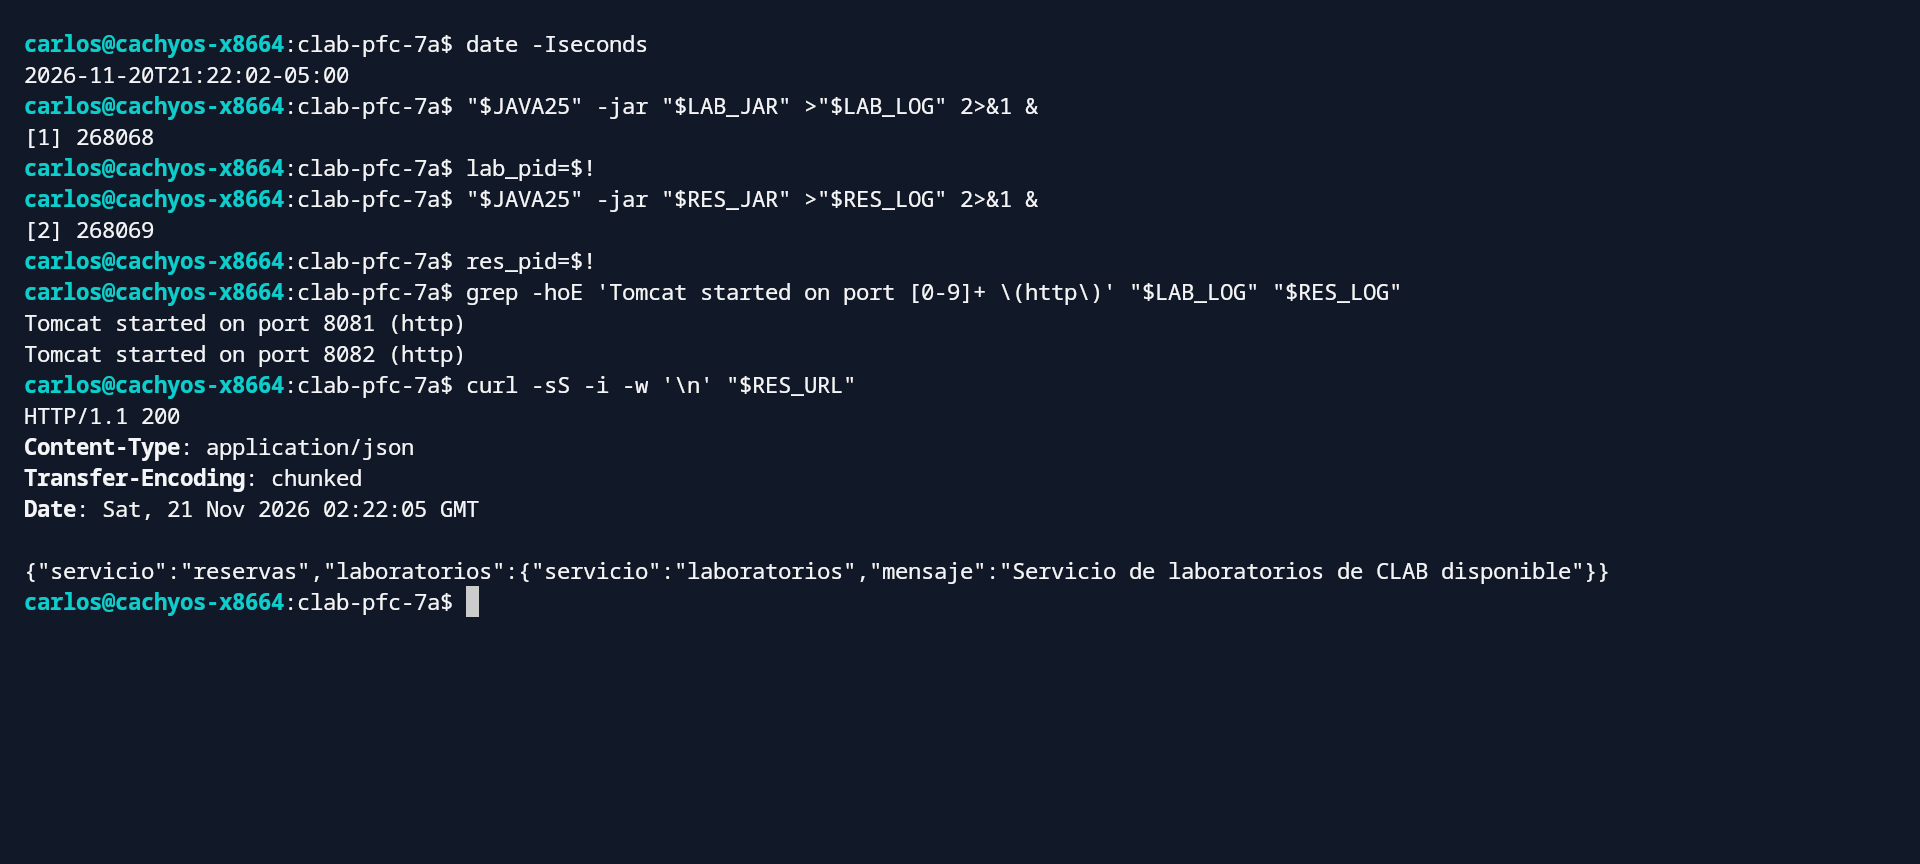
\includegraphics[width=\textwidth]{../evidencias/Laboratorio.png}
    \caption{Arranque de los procesos en los puertos 8081 y 8082 y respuesta
    HTTP 200 de Reservas con el mensaje recibido de Laboratorios.}
  \end{figure*}

  \begin{figure*}[!t]
    \centering
    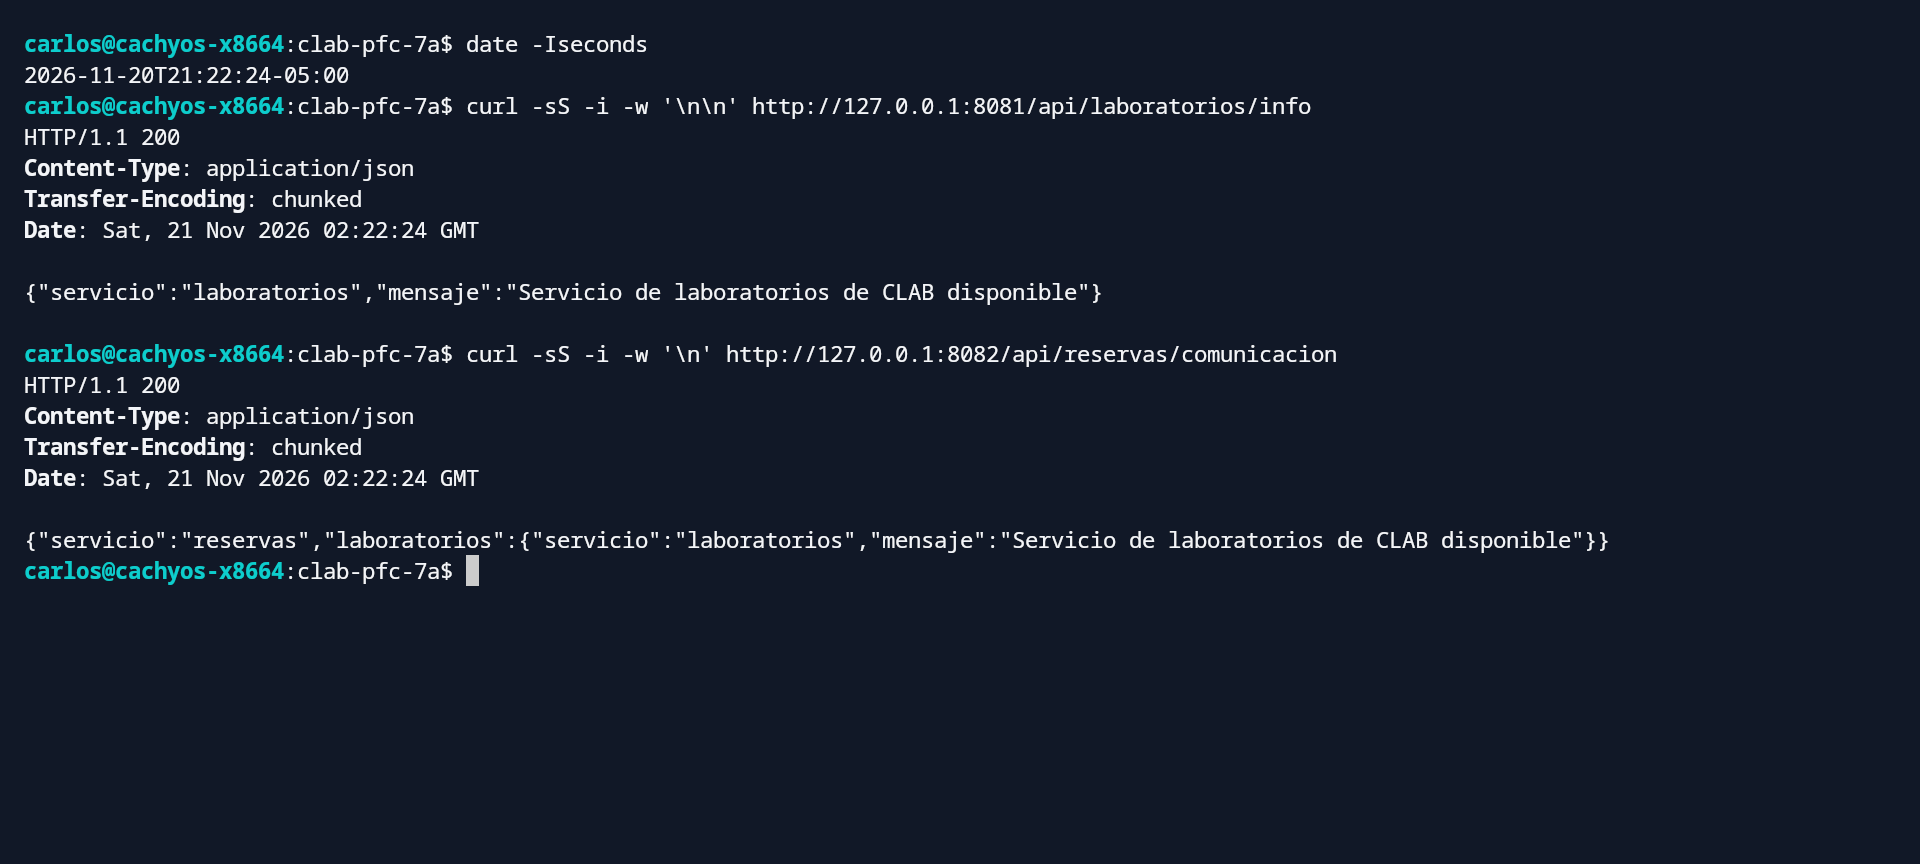
\includegraphics[width=\textwidth]{../evidencias/Consultas.png}
    \caption{Consultas a Laboratorios y Reservas con respuestas HTTP 200 y
    contenido JSON.}
  \end{figure*}

  \begin{figure*}[!t]
    \centering
    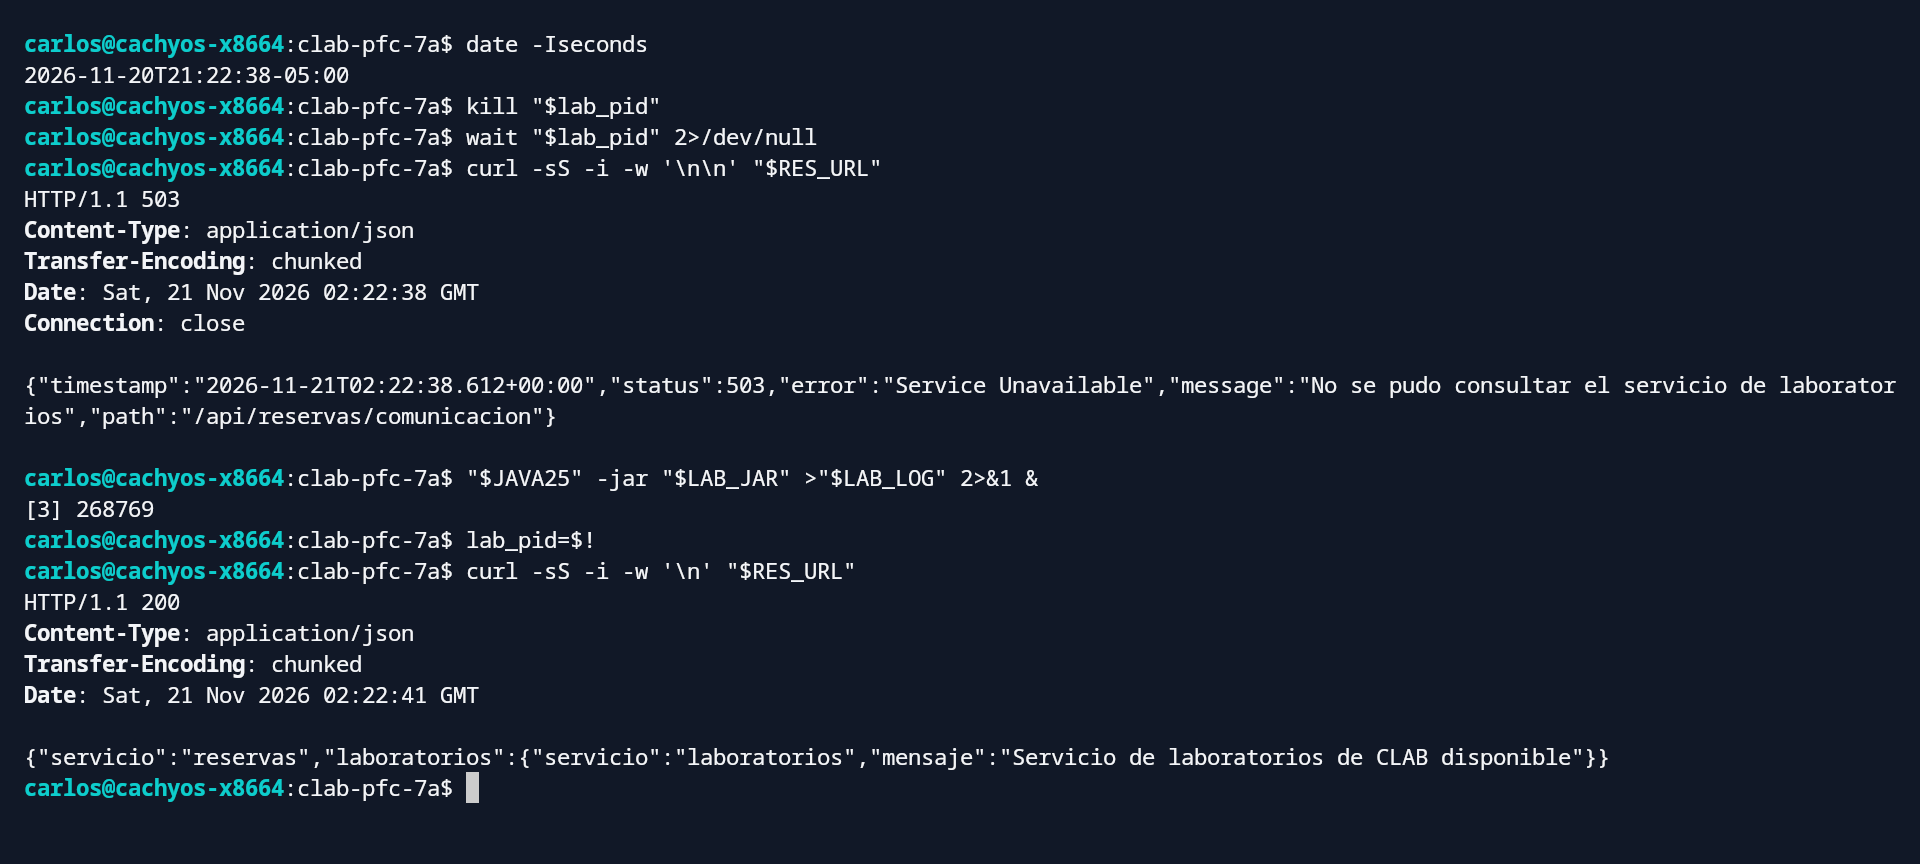
\includegraphics[width=\textwidth]{../evidencias/Reservas.png}
    \caption{Respuesta HTTP 503 al detener Laboratorios y nueva respuesta
    HTTP 200 tras volver a iniciar ese proceso.}
  \end{figure*}
}


\begin{document}

% Documento de integración E1: conservar las contribuciones identificadas.
% Completar solo con información comprobada y aprobada por el equipo.
% Esta estructura no equivale a una entrega terminada.
\ByronPortada
\ByronResumen
\ByronContexto
\ByronObjetivos

\CarlosTrabajosRelacionados

\section{Requisitos}
\ByronHistoriasUsuario

\CarlosRequisitosNoFuncionales

% !TeX root = ../main.tex
\section{Justificación de la arquitectura distribuida}
\label{sec:clab-distribucion}

CLAB parte de una aplicación Angular con backend Spring Boot y persistencia
PostgreSQL. El documento previo identifica reservas coordinadas informalmente,
conflictos de horario, inventario desactualizado e incidencias sin seguimiento.
Estos problemas justifican informatizar el proceso, pero no demuestran por sí
solos que un monolito sea incapaz de resolverlo. No se dispone todavía del acta
firmada o de la grabación consentida que permita verificar el levantamiento
exigido en E1; se usa el documento previo como antecedente, no como evidencia
primaria validada.

La distribución se propone para permitir despliegues por dominio y aislar el
procesamiento de reportes y avisos de la confirmación de reservas. Por ejemplo,
una actualización de estadísticas no debe exigir desplegar de nuevo la agenda;
una caída del servicio de informes no debe deshacer una reserva confirmada.
Un monolito modular es una alternativa viable para la demanda descrita, pero no
ofrece esa independencia de procesos y despliegue. Además, el plan académico
requiere migrar el sistema completo a una base distribuida durante el periodo.
No se usa como justificación una supuesta operación multisede, una saturación
medida o una necesidad de nube pública: ninguna ha sido comprobada.

Los requisitos E1 actuales concretan las metas del antecedente. RNF-01 propone
que al menos el 95\,\% de las consultas válidas de disponibilidad entregue un
resultado correcto en menos de 2 segundos, durante 10 minutos de carga estable
con 50 usuarios concurrentes. Errores y tiempos agotados cuentan como
incumplimientos. RNF-02 propone que al menos el 99\,\% de las comprobaciones de
una sonda por minuto sea correcto dentro de 5 segundos, durante dos semanas
de horario académico acordado. Son umbrales propuestos, no resultados medidos;
la configuración concreta del entorno y su ejecución deben registrarse.

Separar servicios podría permitir escalar consultas e informes sin replicar
toda la aplicación, pero agrega llamadas de red y no prueba esas metas.
La disponibilidad se evalúa por operación: una caída de Avisos no debe impedir
persistir reservas válidas, mientras que perder Identidad impide autorizar
solicitudes protegidas. Un único servidor o una única instancia PostgreSQL
siguen siendo puntos comunes de fallo.

\subsection{Trazabilidad hacia los requisitos E1 actuales}

Se usan los identificadores de la propuesta funcional de \texttt{main.tex}
y los RNF de \texttt{Carlos.tex}, consultados en la revisión
\texttt{a2ecc7d}. No se confunden con los identificadores homónimos del informe
previo, ni se presentan como requisitos ya aprobados o implementados:
\begin{description}
  \item[RF-P01 a RF-P03:] la consulta, solicitud y cancelación se apoyan en
  Reservas como autoridad de ocupación. Laboratorios entrega metadatos y
  estado; Identidad verifica permisos antes de ejecutar cambios.
  \item[RF-P04:] el catálogo pertenece a Laboratorios. Un estado fuera de
  servicio detectado al validar impide una nueva confirmación. Aún debe
  acordarse el instante efectivo del cierre si la desactivación concurre con
  una reserva: consultar el catálogo no hace atómica una operación entre dos
  almacenes. Este punto se registra como pendiente, no como regla ya resuelta.
  \item[RNF-01 y RNF-02:] orientan pruebas de latencia y disponibilidad sobre
  consultas de agenda. La separación permite evaluar el escalado selectivo,
  pero no elimina la dependencia de Identidad o de infraestructura compartida.
  \item[RNF-03:] confirmar, cancelar o bloquear requiere autorización
  verificable. Una revocación o pérdida de Identidad no se sustituye por
  asumir que todo token todavía vigente conserva permisos.
  \item[RNF-04 y RNF-05:] la SPA debe soportar los flujos y tamaños de pantalla
  especificados; los servicios deben poder desplegarse sin nube pública.
  Distribuir no obliga a contratar infraestructura externa.
  \item[RNF-06:] diez solicitudes válidas de la prueba, para franjas libres
  diferentes, deben confirmarse y persistirse con Información y Avisos
  detenido, manteniendo las dependencias de agenda operativas. Los avisos
  quedan fuera de la transacción crítica de confirmación.
  \item[RNF-07:] cada cambio exitoso de agenda del conjunto de prueba requiere
  auditoría en su servicio de origen, incluso si la vista central está caída.
  La copia diferida no sustituye ese registro local.
\end{description}

\subsection{Resumen de ADR-001}

\textbf{Estado: propuesta pendiente de aceptación del equipo.} Se compararon
un monolito modular, doce servicios ---uno por módulo--- y cuatro servicios por
dominio. Se propone la tercera opción para limitar la complejidad operativa:
\begin{itemize}
  \item \textbf{Identidad y Académico:} usuarios, roles, permisos, datos
  académicos y estudiantes.
  \item \textbf{Laboratorios y Recursos:} catálogo, equipos e incidencias.
  \item \textbf{Reservas y Agenda:} reservas, bloqueos y asistencia.
  \item \textbf{Información y Avisos:} reportes de uso, notificaciones y vista
  central de auditoría; la auditoría original permanece en cada dominio.
\end{itemize}

Así se cubren los doce módulos sin exigir doce despliegues. Cada servicio es
dueño de su almacenamiento; no accede a tablas de otro servicio. Reservas
conserva juntas las reservas y los bloqueos para decidir la ocupación en una
transacción local. Se propone que todas las mutaciones de agenda adquieran el
mismo bloqueo de fila por laboratorio antes de comprobar solapamientos y
persistir. La documentación de PostgreSQL distingue restricciones entre filas
de simples comprobaciones locales; una consulta previa aislada no sustituye
la protección concurrente\cite{clabPostgresRestricciones}.

La comunicación REST/JSON ya existe en el esqueleto de E1. El diseño futuro
propone consultas sincrónicas para autorización y validación del catálogo,
y lectura incremental de cambios durables en segundo plano para informes y
avisos. Los contratos y parámetros deben cerrarse en ADR-002 con los resultados
reales de PE-U1, que no estuvieron disponibles en esta revisión. No se atribuye
a REST una superioridad experimental todavía no demostrada.

La migración prevista es incremental: E1 define límites y demuestra dos procesos
comunicándose; E2 incorpora APIs y contenedores; E3 completa la separación de
datos, los módulos restantes y las proyecciones; E4 valida la migración completa,
la recuperación y la calidad. Cada corte mantiene una única fuente de escritura
por entidad y verifica los procedimientos SQL del legado antes de sustituirlos.
El registro completo de opciones, consecuencias y pruebas pendientes está en
\texttt{docs/adr/ADR-001-estilo-arquitectonico.md}.

\paragraph{Estado de implementación y autoría.}
En la revisión del código se identificaron dos servicios mínimos sin persistencia
de negocio. Los cuatro servicios y sus garantías son diseño propuesto, no
integración realizada. Esta sección y ADR-001 se prepararon con asistencia de
IA (OpenAI, GPT-6.1 Sol); no acreditan validación institucional ni aprobación
del equipo.

% !TeX root = ../main.tex
\section{Arquitectura base con el modelo C4}
\label{sec:clab-c4}

El nivel 1 delimita CLAB respecto de las personas y de los sistemas externos;
el nivel 2 lo descompone en aplicaciones y almacenes. En C4, un contenedor no
significa necesariamente un contenedor Docker: también puede ser una SPA, un
servicio o una base de datos\cite{clabC4Contenedores}. Los archivos editables
están en \texttt{docs/diagramas/}; sus figuras vectoriales están en
\texttt{docs/figuras/}.

\subsection{Contexto: nivel 1}

El docente consulta horarios, reserva y reporta fallas; el coordinador planifica
el uso académico; el administrador de laboratorio mantiene recursos y registra
asistencia; el administrador del sistema gestiona accesos y bloqueos. El SGA
se muestra como sistema externo de integración futura, sin conexión activa ni
API acordada; no es una dependencia para ejecutar E1 ni un compromiso de
integración durante el periodo.

\begin{figure*}[!t]
  \centering
  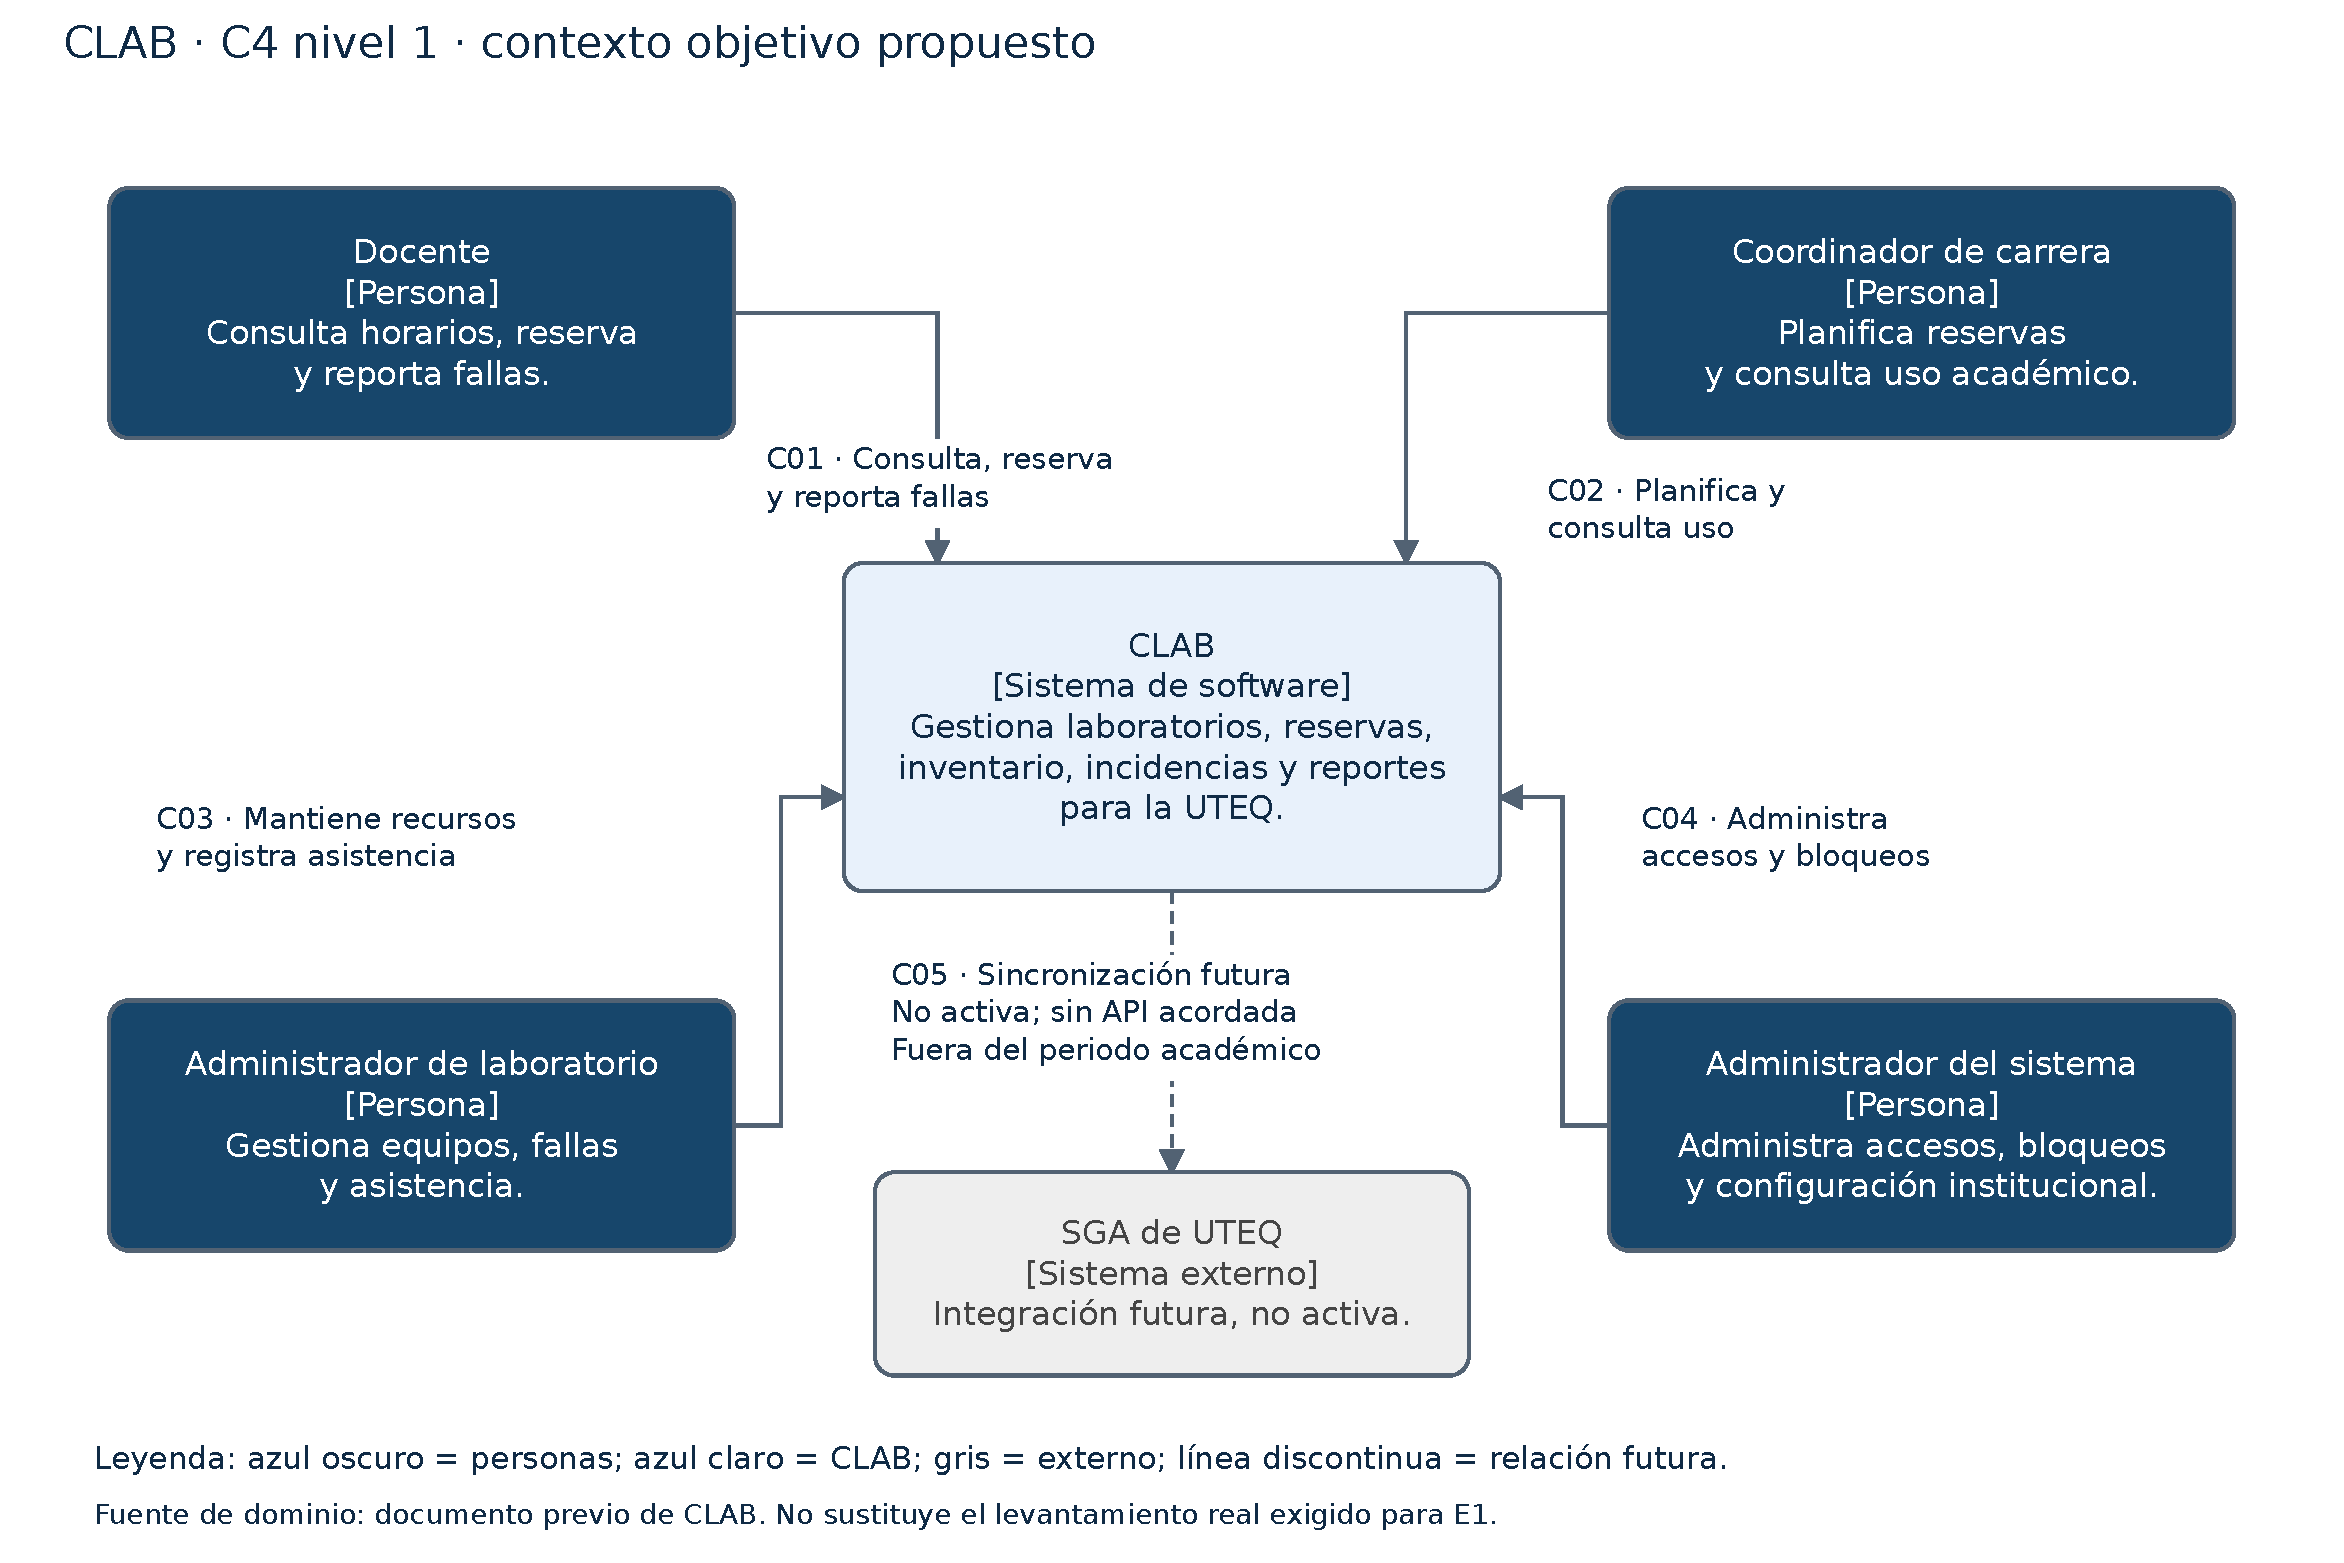
\includegraphics[width=\textwidth,height=0.40\textheight,keepaspectratio]{figuras/c4-contexto.pdf}
  \caption{Contexto objetivo de CLAB. La relación discontinua con el SGA es
  futura, no implementada.}
  \label{fig:clab-contexto}
\end{figure*}

\subsection{Contenedores: nivel 2}

La arquitectura objetivo agrupa los doce módulos del legado en cuatro servicios
con almacenamiento exclusivo, de acuerdo con ADR-001. La SPA no escribe en
bases de datos. No hay consultas SQL entre almacenes ni un broker propuesto
como si estuviera instalado. La auditoría y los cambios se registran localmente
en la transacción de origen, y la vista central los incorpora posteriormente.
La agrupación y los flujos son una propuesta pendiente de aceptación del equipo;
no acreditan que los módulos del backend legado ya se hayan migrado.

\begin{figure*}[!t]
  \centering
  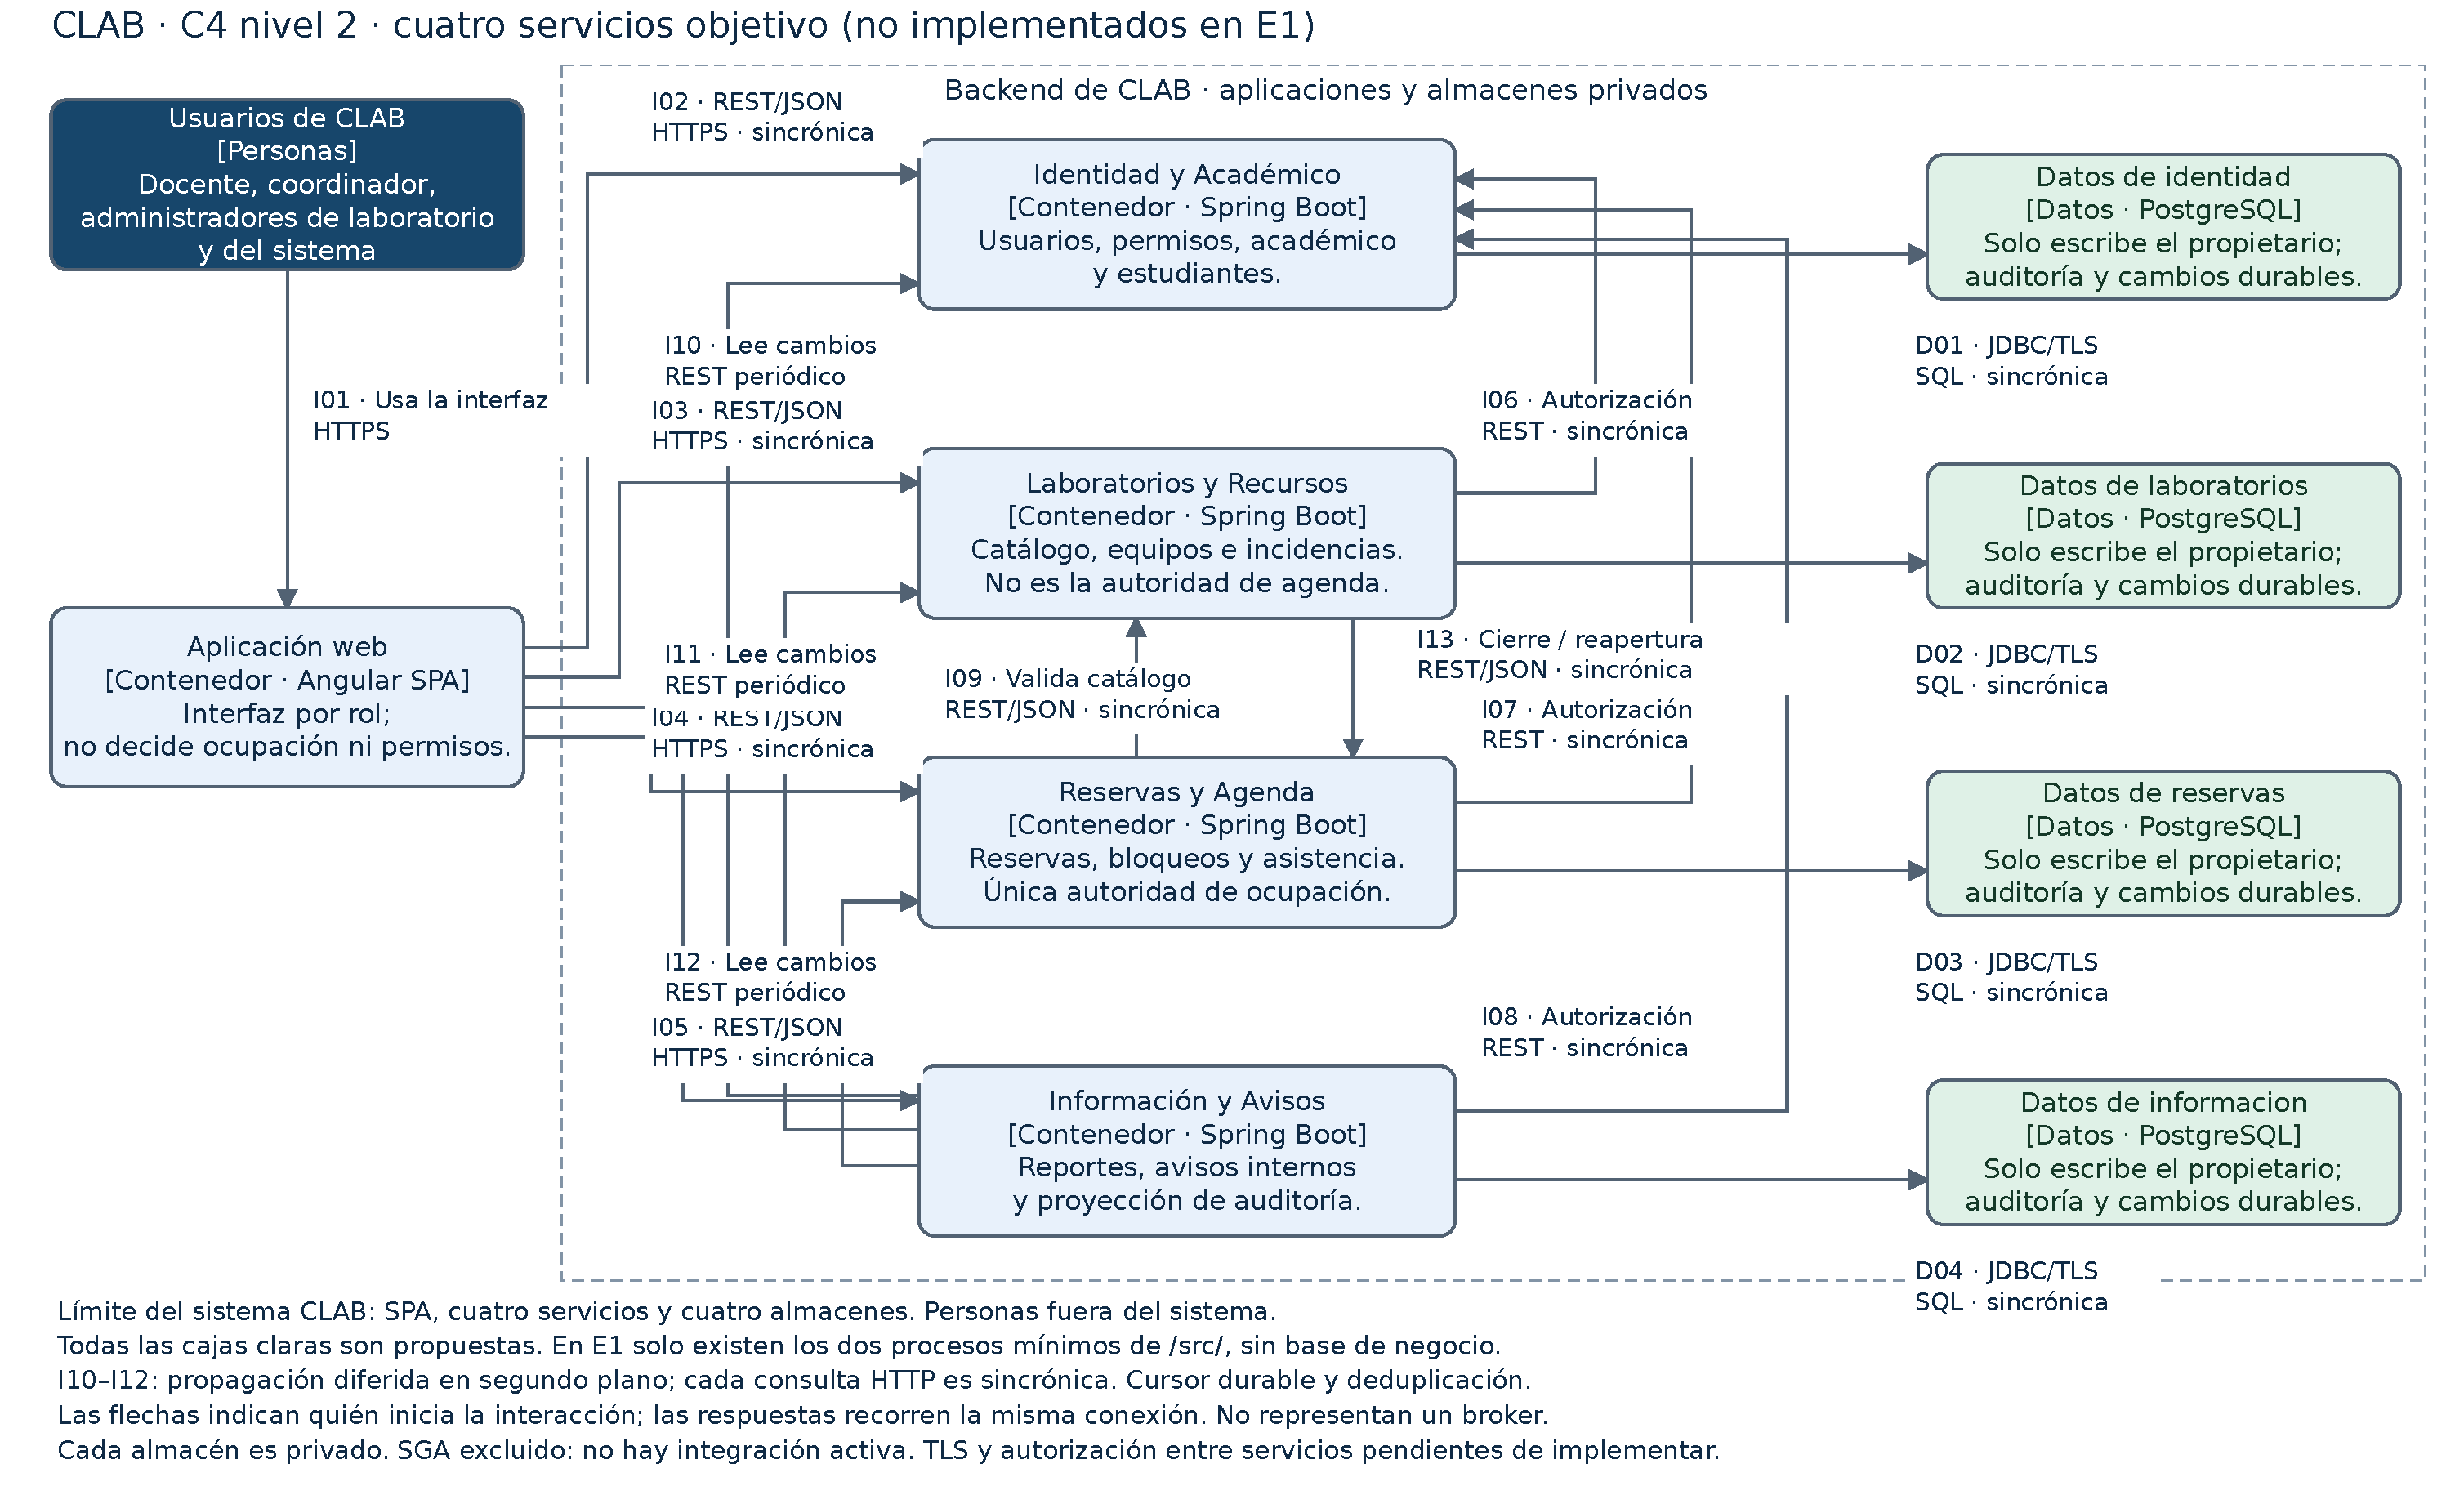
\includegraphics[width=\textwidth,height=0.48\textheight,keepaspectratio]{figuras/c4-contenedores.pdf}
  \caption{Contenedores objetivo de CLAB. Los identificadores permiten
  rastrear las interacciones; no representan funcionalidad implementada en E1.}
  \label{fig:clab-contenedores}
\end{figure*}

\subsection{Lectura y límites de las interacciones}

Las flechas indican el iniciador; la respuesta vuelve por la misma conexión.
Los identificadores son un inventario de interfaces de arquitectura para
contrastarlo con el modelo de comunicación y ADR-002, no una sustitución de
esos entregables.

\begin{description}
  \item[I01:] personas a SPA por HTTPS.
  \item[I02--I05:] SPA a Identidad, Laboratorios, Reservas e Información,
  respectivamente, mediante REST/JSON sincrónico sobre HTTPS. Cada servicio
  aplica permisos; ocultar un botón en Angular no es autorización.
  \item[I06--I08:] Laboratorios, Reservas e Información consultan Identidad
  mediante REST sincrónico para autorizar peticiones protegidas. Si Identidad
  no responde, no se autoriza la operación; esto introduce un punto común de
  dependencia que deberá medirse.
  \item[I09:] Reservas valida el catálogo de Laboratorios mediante REST/JSON
  sincrónico antes de confirmar una nueva reserva. La ocupación se decide en
  Reservas, no con una copia del calendario en Laboratorios.
  \item[I10--I12:] Información consulta los cambios de Identidad, Laboratorios
  y Reservas, respectivamente, mediante REST periódico. La incorporación a
  reportes y avisos es diferida: cada HTTP espera respuesta, pero la transacción
  original no espera que la proyección se actualice. Cursores, retención,
  autenticación de máquina y reintentos todavía requieren implementación.
  El contrato de cambios debe limitarse a los datos necesarios para cada
  proyección: no debe exponer contraseñas, hashes, tokens ni secretos de sesión.
  \item[I13:] Laboratorios solicita a Reservas el cierre o la reapertura de
  la barrera operativa mediante REST/JSON sincrónico, con identificador estable
  y revisión. Reservas autoriza y persiste el cambio sin volver a llamar a
  Laboratorios desde este manejador. Ante un resultado desconocido se consulta
  o reintenta la misma solicitud; no se infiere que haya fallado por un timeout.
  \item[D01--D04:] cada servicio accede únicamente a su propio almacén mediante
  JDBC y SQL, con TLS previsto para conexiones de red. Persistencia y registros
  de cambios durables no están presentes en los dos servicios mínimos de E1.
\end{description}

No se propone invocar servicios de negocio desde Información para ejecutar
escrituras. Si Información está detenido, la agenda debe poder confirmar y
mantener sus registros locales. Si Laboratorios o Identidad están inaccesibles,
una nueva reserva que dependa de ellos no se confirma. Esto es aislamiento
parcial por operación, no disponibilidad total frente a cualquier fallo.

Para RF-P04, Laboratorios solo publica fuera de servicio después de confirmar
la barrera en Reservas; en caso contrario muestra cierre pendiente. La barrera
se verifica bajo el mismo bloqueo por laboratorio que cada confirmación de
reserva. Las reservas previas se conservan, sin cancelación automática ni
autorización de uso físico del espacio cerrado. Para reabrir, el catálogo pasa
primero a apertura pendiente, después Reservas retira únicamente su barrera
operativa y finalmente el catálogo publica activo. Un fallo no debe provocar
que se anuncie un cierre sin barrera o una reapertura sin confirmación.
Los estados, revisiones y reintentos de este diseño se detallan en ADR-001.

\subsection{Correspondencia con el esqueleto de E1}

En el código revisado existen \path{servicio-reservas} y
\path{servicio-laboratorios}. La petición
\path{/api/reservas/comunicacion} consulta
\path{/api/laboratorios/info} por HTTP y devuelve el mensaje recibido.
Esa relación es el antecedente técnico de I09, pero todavía no valida un
laboratorio real ni crea reservas. Los procesos se enlazan a la interfaz local;
HTTPS, autorización, bases privadas y propagación de cambios son diseño futuro.
No se ha ejecutado ni validado la arquitectura completa de cuatro servicios.

\paragraph{Evidencia de diseño y asistencia.}
Estos diagramas digitales no sustituyen el primer bosquejo ni las dos
fotografías reales de sesiones del equipo. Se prepararon con asistencia de
IA (OpenAI, GPT-6.1 Sol); no acreditan participación presencial ni sesiones
que no estén documentadas por los integrantes.

% !TeX root = ../main.tex
% Base: borrador de JulianaEmanuel, commit 85e7c67. Se conservan sus políticas,
% la etiqueta original y la referencia clabAbadiPACELC2012; se amplía el análisis.
% Asistencia del borrador base: OpenAI Codex. Ampliación: OpenAI GPT-6.1 Sol.
\section{Análisis CAP y PACELC}
\label{sec:clab-cap}
\label{sec:clab-cap-pacelc}

CAP expresa que, bajo una partición, no se pueden garantizar simultáneamente
consistencia linealizable y respuesta satisfactoria para todas las solicitudes
dirigidas a nodos no fallidos\cite{clabGilbertLynchCAP}. Su disponibilidad no es
el porcentaje mensual de disponibilidad de un requisito no funcional. Tampoco
la consistencia de CAP equivale simplemente a las restricciones de integridad
de ACID. PACELC añade el compromiso, cuando no hay partición, entre latencia y
consistencia\cite{clabAbadiPACELC2012,clabAbadiPACELC}.

CLAB todavía no tiene replicación de negocio en el esqueleto de E1. Por eso no
se etiqueta PostgreSQL ni todo el sistema como ``CP'' o ``AP'' por su nombre.
Se especifican políticas objetivo por operación: \textbf{PC/EC} prefiere
consistencia bajo partición y también en operación normal; \textbf{PA/EL} permite
lecturas de una proyección local potencialmente atrasada y prioriza la latencia.
La segunda política solo mantiene lectura en los nodos que tengan una copia
accesible; no promete disponibilidad universal ni escritura multimaestro.

\subsection{Relación con los requisitos E1}

Se emplean los identificadores actuales de \texttt{main.tex} y
\texttt{Carlos.tex}, revisados en \texttt{b212d70}. RF-P02 exige como máximo
una confirmación ante dos solicitudes simultáneas para el mismo laboratorio
y horario. RNF-03 exige impedir cambios si no hay permiso verificable, si la
sesión está revocada o si Identidad no puede verificarla. Ambos orientan la
preferencia por consistencia en el camino de confirmación.

RNF-01 propone al menos el 95\,\% de consultas válidas de disponibilidad
correctas en menos de 2 segundos durante 10 minutos con 50 usuarios concurrentes.
RNF-02 propone al menos el 99\,\% de comprobaciones correctas dentro de 5 segundos,
con una sonda por minuto durante dos semanas de horario académico. Son metas
de evaluación, no valores medidos ni garantías deducidas de CAP. RNF-06 y
RNF-07 requieren confirmar y persistir las reservas de prueba con Avisos detenido
y mantener auditoría fuente de todos los cambios exitosos, respectivamente.

\subsection{Reservas y bloqueos de agenda: PC/EC}

\textbf{Dato e invariante.} El servicio Reservas es la única autoridad de
ocupación: dos reservas confirmadas no pueden solaparse para el mismo laboratorio;
un bloqueo confirmado impide nuevas reservas dentro de su intervalo. Un bloqueo
que afecta reservas existentes debe registrar las afectaciones en la misma
transacción. El catálogo de Laboratorios no es una segunda agenda.

\textbf{Con partición.} Si el solicitante no llega a la autoridad de agenda o
esta no puede confirmar sus dependencias de autorización y catálogo, no recibe
una confirmación nueva. No se aceptan reservas sin conexión para fusionarlas
después: el usuario debe reintentar y puede perder el horario. Un calendario
almacenado previamente, si se muestra, es informativo y no concede el intervalo.

\textbf{Sin partición.} La confirmación espera la transacción autoritativa.
Se propone serializar por laboratorio todas las reservas, bloqueos, cancelaciones
y recurrencias mediante un bloqueo de fila estable. Intervalos contiguos
se interpretan como $[inicio,fin)$: se permite que uno termine cuando comienza
el siguiente. Se sacrifica latencia frente a confirmar desde una copia atrasada.
La garantía debe probarse con concurrencia, no inferirse de usar
\texttt{@Transactional}.

\textbf{Recuperación.} Un timeout no prueba que la transacción haya fallado.
Se propone una clave de idempotencia por solicitud, registrada con la operación,
y una consulta del resultado antes de reintentar. El diseño de API aún debe
implementarse; el endpoint de comprobación de E1 no crea reservas.

\subsection{Usuarios activos, roles y permisos: PC/EC}

Identidad es la fuente de verdad de credenciales y autorizaciones. Los otros
servicios consultan su validación antes de aceptar peticiones protegidas.
Durante una partición con Identidad se rechaza temporalmente la operación;
no se presume que un token aún vigente mantenga permisos ya revocados.
Sin partición se paga una llamada adicional para verificar usuario activo y
permisos. Sigue pendiente acordar el efecto de una revocación que coincida con
una operación ya autorizada; no se promete anular retroactivamente una
transacción confirmada. Esta dependencia reduce disponibilidad y debe incluirse
en las pruebas y en la estimación del 99\,\% de disponibilidad.

\subsection{Catálogo, equipos e incidencias: autoridad PC/EC}

Laboratorios y Recursos decide actualizaciones de catálogo, estado operativo e
incidencias. Si no se llega a su almacén autoritativo no se confirman cambios
ni cierres de incidencias. Sin partición se confirma después de persistir el
cambio y su auditoría local. Esto impide que dos copias aisladas comuniquen
estados contradictorios como definitivos. La pérdida de este servicio no borra
reservas existentes, pero bloquea nuevas confirmaciones que necesiten validar
el catálogo. El cierre por mantenimiento requiere además un bloqueo de agenda
confirmado en Reservas; actualizar solamente un campo del catálogo no garantiza
el cierre del intervalo. No se promete atomicidad entre ambos servicios.

Para RF-P04 se propone que Laboratorios persista cierre pendiente y solicite
por I13 una barrera de admisión en Reservas. Solo publica fuera de servicio
después de confirmar durablemente esa barrera. Cada confirmación de reserva
la comprueba bajo el mismo bloqueo local, aunque una consulta previa haya leído
un catálogo activo. Una reserva confirmada antes de la barrera se conserva;
una confirmación posterior se rechaza. No se cancelan automáticamente reservas
existentes ni se autoriza con ello el uso físico de un laboratorio cerrado.

Durante una partición, el trámite no se anuncia completado sin confirmación.
Si la barrera se activó y se perdió la respuesta, el catálogo puede seguir
pendiente mientras Reservas rechaza nuevas confirmaciones. Se prefiere perder
disponibilidad antes que reabrir por una compensación insegura. La recuperación
consulta o reintenta la misma solicitud durable; identificador y revisión
evitan duplicados y órdenes anteriores aplicadas fuera de secuencia.

La reapertura comienza cambiando el catálogo a apertura pendiente, todavía
no reservable, y después retira la barrera operativa mediante I13. Solo tras
confirmar esa revisión publica activo. No retira otros bloqueos de agenda.
Una respuesta perdida conserva la apertura pendiente, no un retorno automático
a fuera de servicio con una barrera que pudiera estar retirada. Sin partición
se acepta la latencia de estas dos confirmaciones locales; no se promete una
transacción distribuida atómica. El protocolo completo queda en ADR-001 y aún
debe implementarse y validarse con el equipo.

\subsection{Asistencia y datos académicos: autoridad PC/EC}

Reservas registra asistencia únicamente para una reserva válida; Identidad y
Académico mantiene estudiantes, matrículas, periodos y asignaturas. Las escrituras
requieren acceso al servicio propietario y autorización vigente. Durante una
partición no se confirma una asistencia o matrícula solo desde el navegador.
Sin partición se prioriza la persistencia autoritativa sobre responder desde
una copia local. Una reserva puede conservar una instantánea de sus metadatos
académicos para explicar el registro histórico, sin convertirla en fuente de
verdad de matrículas o permisos.

\subsection{Auditoría: fuente PC/EC y vista central PA/EL}

La operación de negocio y su auditoría fuente se guardan en una transacción
local: si no puede registrarse esa auditoría obligatoria, no se confirma el
cambio. La copia central en Información y Avisos se alimenta posteriormente.
Durante una partición entre servicios, la copia central puede seguir mostrando
los eventos ya recibidos, con su marca de última actualización; no certifica
que incluya toda la actividad actual. Sin partición se prefiere leer esa
proyección sin consultar todos los orígenes en cada pantalla. La convergencia
requiere recuperación de registros durables y deduplicación, no entrega
``exactamente una vez'' supuesta.

\subsection{Reportes y notificaciones: proyecciones PA/EL}

Información y Avisos puede consultar su copia local aunque no lleguen cambios
de Reservas o Laboratorios. El usuario verá estadísticas atrasadas o recibirá
la notificación después; ninguna de esas vistas confirma disponibilidad de
horarios. En operación normal se conserva la lectura local para reducir latencia.
El atraso no tiene una cota demostrada: depende de la frecuencia de consulta,
el volumen pendiente y las interrupciones. Tras restablecer la conexión, se
reanuda desde cursores persistidos y se deduplican los cambios. Si el propio
servicio, su almacén o Identidad están inaccesibles, la consulta protegida no
queda disponible por llamarla PA/EL.

\subsection{Alcance de las garantías y comprobaciones pendientes}

Un único escritor por dominio simplifica la autoridad, pero no es una solución
de alta disponibilidad. Si en E3 se añaden réplicas para datos críticos, deberán
definirse replicación, confirmación durable y elección de primario con protección
contra dos escritores simultáneos; una promoción manual sin verificar ese
aislamiento no demuestra consistencia. Las políticas anteriores orientan ese
diseño y no acreditan un protocolo de consenso implementado. La replicación
debe preservar el orden de confirmación incluso al cambiar el nodo responsable.

La validación prevista debe comprobar: dos solicitudes concurrentes para el
mismo intervalo; reserva simultánea con bloqueo; pérdida de respuesta tras una
confirmación; desactivación concurrente de RF-P04; revocación de permisos;
corte y recuperación de los canales de
proyección; reinicio del consumidor conservando cursores; y fallo de la
persistencia de auditoría. Para los intervalos iguales, el criterio propuesto
es como máximo una confirmación y un resultado explícito para la otra solicitud.
Para la proyección, el criterio es convergencia sin pérdida ni duplicación
observable después de recuperar los cambios conservados en el origen.

\paragraph{Estado.}
Este análisis amplía el borrador incorporado por JulianaEmanuel en el commit
\texttt{85e7c67}, preparado con OpenAI Codex, conservando sus políticas de agenda,
autorización y proyecciones y su referencia de PACELC. La ampliación se preparó
con asistencia de IA (OpenAI, GPT-6.1 Sol) y se contrasta con ADR-001 y los
contenedores objetivo. No se ejecutaron
experimentos de partición, concurrencia ni replicación del sistema de negocio
durante su preparación. Sus efectos deben contrastarse con requisitos trazables
al levantamiento real y con la implementación posterior.


\CarlosRiesgosTecnicos

\ByronTablaAportes

\section{Declaración de uso de inteligencia artificial}
\CarlosDeclaracionIA
\ByronDeclaracionIntegracion
\ByronDeclaracionesRegistradas

\ByronEvidenciasEsqueleto

\printbibliography[heading=bibnumbered,title={Referencias}]

\end{document}
